\documentclass[11pt,a4paper]{article}
\usepackage[UTF8,fontset=none]{ctex}
\usepackage{fontspec}
\setmainfont{DejaVu Serif}
\setsansfont{DejaVu Sans}
\setCJKmainfont{Noto Serif CJK SC}
\setCJKsansfont{Noto Sans CJK SC}
\setCJKmonofont{Noto Sans Mono CJK SC}
\usepackage[a4paper,left=21mm,right=21mm,top=20mm,bottom=20mm,headheight=14pt,headsep=8mm]{geometry}
\usepackage{graphicx,booktabs,tabularx,array,amsmath,amssymb}
\usepackage{xcolor,titlesec,fancyhdr,caption,hyperref,microtype,placeins,pdflscape,float,etoolbox}
\usepackage{longtable,enumitem,needspace}
% Repository adapter: the supplied portable definitions remain in the immutable
% source ZIP. Run XeLaTeX from task1/reports/experiment1 as build.sh does.
% Smart Cities & Location Services — P2 Cloud Sorbet
% LOCKED visual palette v1 for Experiment Report
\definecolor{Paper}{HTML}{FCFAF7}
\definecolor{Ink}{HTML}{2D3238}
\definecolor{Muted}{HTML}{70757A}
\definecolor{P1}{HTML}{D3EAF5} % light blue
\definecolor{P2}{HTML}{F5D9B8} % apricot
\definecolor{P3}{HTML}{E8C7D3} % soft rose
\definecolor{P4}{HTML}{D7D3EA} % mist violet
\definecolor{C1}{HTML}{5B9FBE} % blue accent
\definecolor{C2}{HTML}{D49757} % apricot accent
\definecolor{C3}{HTML}{B97589} % rose accent
\definecolor{C4}{HTML}{8177A8} % violet accent
\definecolor{Rule}{HTML}{DDE3E7}
\definecolor{Panel}{HTML}{FFFDFC}


\pagecolor{Paper}\color{Ink}
\hypersetup{colorlinks=true,linkcolor=C1,urlcolor=C1,citecolor=C4,
 pdftitle={实验一：轨迹预处理与质量评估},pdfauthor={吴博闻 / 10245102410},
 pdfsubject={分段、方向去噪与简化的结果驱动比较}}
\linespread{1.20}
\setlength{\parindent}{2em}\setlength{\parskip}{.28em}
\setlength{\emergencystretch}{2em}
\clubpenalty=10000\widowpenalty=10000
\titleformat{\section}[hang]{\sffamily\bfseries\Large}{\color{C1}\fontsize{25}{27}\selectfont\thesection}{.65em}{}
\titleformat{\subsection}{\sffamily\bfseries\large}{\thesubsection}{.65em}{}
\titlespacing*{\section}{0pt}{1.3em}{.7em}
\titlespacing*{\subsection}{0pt}{1.1em}{.5em}
\pagestyle{fancy}\fancyhf{}
\fancyhead[L]{\sffamily\small\color{Muted}智慧城市与位置服务}
\fancyhead[R]{\sffamily\small\color{Muted}Experiment Report}
\fancyfoot[C]{\sffamily\small\color{Muted}\thepage}
\renewcommand{\headrulewidth}{0pt}
\captionsetup{font=small,labelfont={bf,sf},labelsep=quad,skip=5pt}
\newcolumntype{L}[1]{>{\raggedright\arraybackslash}p{#1}}
\newcolumntype{Y}{>{\raggedright\arraybackslash}X}
\newcolumntype{Z}{>{\centering\arraybackslash}X}
\setlength{\tabcolsep}{5pt}
\renewcommand{\arraystretch}{1.22}
\setlist{nosep,leftmargin=2em}
\newcommand{\tabnote}[1]{\par\vspace{2mm}\begin{minipage}{\linewidth}\footnotesize\color{Muted}#1\end{minipage}}
\newcommand{\nextchapter}{\FloatBarrier\clearpage}
\setcounter{tocdepth}{1}
\pretocmd{\subsection}{\Needspace{9\baselineskip}}{}{}
\raggedbottom
\setlength{\textfloatsep}{14pt plus 2pt minus 2pt}
\setlength{\intextsep}{12pt plus 2pt minus 2pt}
\begin{document}
\hypersetup{pageanchor=false}
\begin{titlepage}\thispagestyle{empty}\setlength{\parindent}{0pt}
\vspace*{21mm}
{\sffamily\small\bfseries\color{C1}SMART CITIES \& LOCATION SERVICES}\par
\vspace{14mm}{\sffamily\fontsize{17}{23}\selectfont 实验一}\par
\vspace{5mm}{\sffamily\bfseries\fontsize{27}{36}\selectfont 轨迹预处理与质量评估}\par
\vspace{5mm}{\large 分段、方向去噪与简化的结果驱动比较}\par
\vspace{17mm}\noindent{\color{Rule}\rule{\linewidth}{.8pt}}\par
\vspace{12mm}\renewcommand{\arraystretch}{1.7}
\begin{tabular}{@{}l@{\hspace{12mm}}l@{}}
\textsf{\textcolor{Muted}{姓名}} & 吴博闻\\[2mm]
\textsf{\textcolor{Muted}{学号}} & 10245102410\\[2mm]
\textsf{\textcolor{Muted}{课程}} & 智慧城市与位置服务\\[2mm]
\textsf{\textcolor{Muted}{日期}} & 2026年9月29日
\end{tabular}
\vfill{\sffamily\small\color{Muted}Experiment Report}\par\vspace{4mm}
\noindent{\color{P1}\rule{.34\linewidth}{3pt}\color{P2}\rule{.22\linewidth}{3pt}\color{P3}\rule{.20\linewidth}{3pt}\color{P4}\rule{.14\linewidth}{3pt}}\par\vspace*{8mm}
\end{titlepage}
\hypersetup{pageanchor=true}\pagenumbering{roman}
\section*{实验概述}
本报告介绍轨迹分段、方向去噪和 Douglas--Peucker（DP）简化的实现与评价，并比较参数、处理顺序及 LLM 辅助方式对结果的影响。实验先检查单项调整的作用，再检验组合是否带来额外收益；方案确定后，使用预先保留的记录进行确认，最后处理全部轨迹。各项选择均依据实际结果，而不预设更复杂的方案一定更好。
\vspace{8mm}
\tableofcontents
\clearpage\pagenumbering{arabic}
\section{数据与实验思路}
\subsection{先区分采样现象与位置错误}
课程提供的轨迹数据\cite{teacher}包含11,386条记录，共1,173,410个观测点。每条记录由相互对应的时间序列和坐标序列组成，记录内共有1,162,024对相邻观测。文件中的记录键用于区分这些序列，并不提供用户身份或完整行程信息。

选择处理方法之前，需要先看清数据中出现了什么。全量检查得到表\ref{tab:data}中的四类现象。相邻坐标完全相同的情况较多；同时，也存在时间差为零但坐标不同，以及采样间隔超过30秒的情况。这些统计描述的是观测特征，不是已经标注好的噪声类别。

\begin{table}[htbp]\centering
\caption{原始轨迹的部分采样现象}\label{tab:data}
\small\renewcommand{\arraystretch}{1.28}
\begin{tabularx}{\linewidth}{@{}Yrr@{}}\toprule
相邻观测的特征 & 数量 & 占相邻观测对的比例\\\midrule
位置完全相同 & 575,278 & 49.51\%\\
时间差为零 & 42,185 & 3.63\%\\
同一时刻、不同位置 & 29,175 & 2.51\%\\
时间差超过30秒 & 8,272 & 0.71\%\\\bottomrule
\end{tabularx}
\vspace{3.5mm}
\begin{minipage}{\linewidth}\footnotesize\color{Muted}
统计单位为同一记录内的相邻观测对，比例分母均为1,162,024。不同现象可能重叠，数量不能相加作为异常点总数；30秒在此用于描述采样间隔，是否适合作为分段阈值将在后文比较。
\end{minipage}
\end{table}

\subsection{直接连线与直接删点各有什么风险}
若把所有相邻观测直接连接，较长的采样空档也会被画成一条连续线段，而空档期间的实际路径并未被记录。另一方面，相同坐标在不同时间出现，可能包含停留信息，不能仅因位置重复就直接删除。同一时刻出现不同位置时，相邻速度也无法由距离除以时间差得到；实验保留这种不可计算情况，而不是把速度填成零。

局部方向突变同样需要进一步检查：它可能来自位置异常，也可能是真实折返。分段、方向去噪与简化分别面对连接、局部形状和点数冗余问题，不能只凭轨迹看起来更平滑，就认定处理更准确。

\clearpage
\subsection{把空间位置与采样时间一起观察}
只看二维连线，相同位置的多次观测容易叠在一起。图\ref{fig:space-time}将记录352的170个观测点沿相对时间展开，并叠加后文最终方案的处理结果，便于同时观察采样先后、片段连接和保留点的位置。本例用于解释处理关系，整体效果仍由后续样本与全量结果判断。

\begin{figure}[htbp]\centering
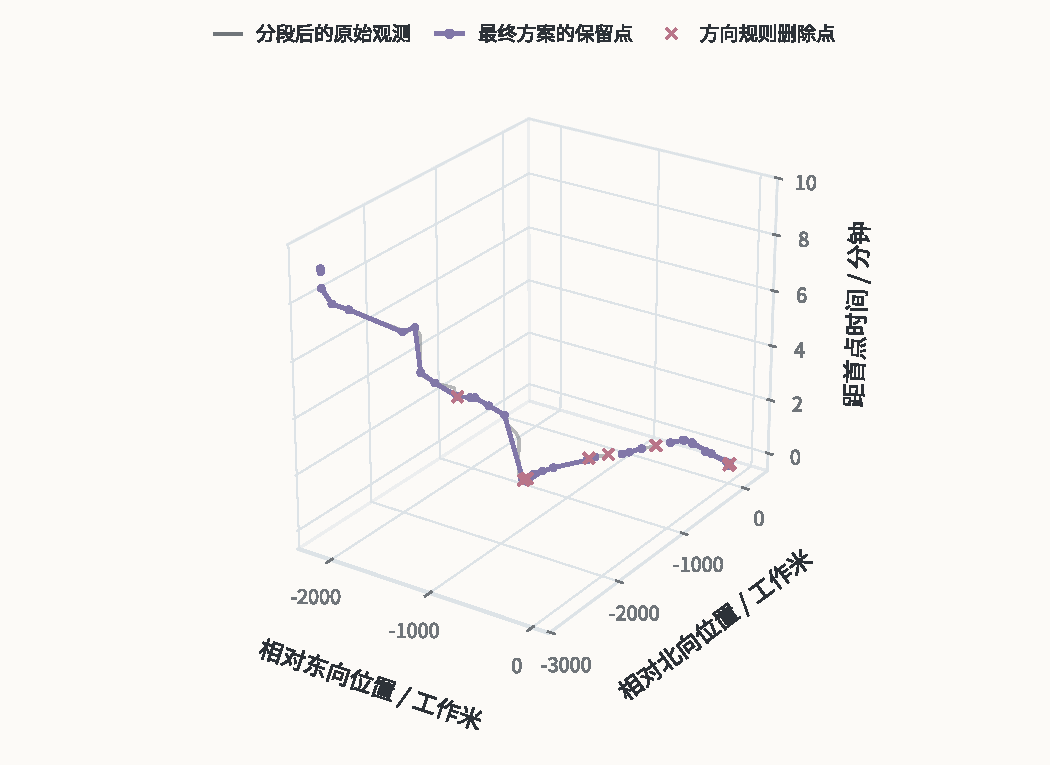
\includegraphics[width=.98\linewidth]{figures/G1A_space_time.pdf}
\caption{记录352的三维时空表示。灰线为分段后的原始观测，紫线连接最终方案保留的点，叉号标出方向规则删除点；各片段之间不连线。空间位置仅平移至首点，竖轴为相对时间而非海拔，也不参与平面距离计算。}\label{fig:space-time}
\end{figure}

数据文件未注明坐标参考系。实验使用固定椭球模型，将经纬度数值转换至同一局部平面，统一计算距离和方向。下文以“工作米”表示这一模型中的长度，用于方案间比较，不代表已经确认的真实定位精度；具体转换与核对方法放在方法说明及附录中。

\subsection{怎样从处理结果中选择方案}
仅看删除数量，容易奖励丢弃大量数据的方案；仅看最后一步的误差，又可能忽略前面已经删除的点。因此，实验先核对各步骤是否按定义执行，再使用同一原始参考比较覆盖、几何偏差和压缩效果。局部检查合格，是继续比较的前提，不是采用方案的充分理由。

后续先分别改变参数与处理顺序，保留各项独立结果；有依据的调整才进一步组合。LLM提出的设置也进入相同的处理和核验过程。结果满足比较条件时继续验证，出现退化则保留原方案；实现错误修正后重算，方法没有收益则如实记录。下一章先说明三种处理操作及其检查方式，再展开方案之间的比较。


\nextchapter\section{轨迹预处理与评价方法}
\label{sec:method}

\subsection{何时应将相邻观测断开}
采样空档两端的观测只能说明两个时刻的位置，不能说明中间走过的路径。因此，分段首先处理不可靠的连接，而不是立即判断某个端点是否错误。

记第$i$个观测的工作平面坐标为$p_i=(E_i,N_i)$，时间为$t_i$。当前相邻观测满足
\[
\Delta t_i=t_{i+1}-t_i>\tau_t,\qquad
\Delta t_i<0,\qquad\text{或}\qquad
\|p_{i+1}-p_i\|>\tau_d
\]
中的任一条件时，在右侧点之前断开。等于阈值时不切分，右点只归入新片段。原始数据未出现负时间差，这一情况仍保留为输入检查。时间差为零不单独触发时间切分，也不被填成可计算的速度。

切开后的短片段是否还值得继续处理，是另一个问题。参考设置过滤点数少于$n_{\min}$或累计长度小于$L_{\min}$的片段；累计长度只加总段内相邻边，不包含已经切断的连接。将切分和过滤分开，才能辨认信息是在断点处失去连接，还是在过滤时被整段舍弃。下文用S表示这两个连续操作。

参考条件是否合适，需要后面的参数实验判断。这里首先核对每个原始点的片段归属、边界位置和过滤原因，并检查输出是否重新跨过原始断点。相同点不能因切分重复出现在两个片段，过滤掉的记录也继续计入结果分母。

\subsection{怎样检查方向突变，而不将它直接当作噪声}
方向突然改变可能来自位置偏移，也可能是真实折返。实验以课程给定的双侧方向关系\cite{teacher}识别待检查点，而不把方向变化预先视为噪声标签。

对非零位移边，定义当前点到下一点的出边方向：
\[
\alpha_i=\left[\frac{180}{\pi}\operatorname{atan2}(E_{i+1}-E_i,N_{i+1}-N_i)\right]\bmod 360^\circ.
\]
方向差采用环形角差$\delta(a,b)=\min(|a-b|,360^\circ-|a-b|)$。若
\[
\delta(\alpha_i,\alpha_{i-1})>\theta
\quad\text{且}\quad
\delta(\alpha_i,\alpha_{i+1})>\theta,
\]
则标记点$i$。这里比较相邻出边方向，需要相应的前后观测；它不是把任意三点的一个内角与阈值比较。

若边遍历边删除，前面的动作会改变后续邻域，结果可能依赖遍历次序。实验先在本阶段完整输入上计算全部标记，再同时删除，不迭代至不再能删。首尾、缺少必要后继或零位移导致方向不可计算的窗口保留并标明原因。此后重新计算相邻关系，避免把删除前的方向和长度继续用于下一步。

核验时逐个检查实际删除点是否满足这次输入上的谓词。构造折返和尖峰例子则用于检查规则的解释边界：\textbf{正确执行方向规则，与准确辨认真实噪声不是同一个判断。}这一步记为D。

\subsection{怎样减少点数并控制简化偏差}
短时间内的重复或近共线观测会增加存储量，但任意删点又可能拉直转弯。DP的做法是先用端点连线近似一段轨迹，若中间点偏离过大，就保留最远点，并分别处理左右两段\cite{teacher}。

对于端点$a,b$与中间点$p$，投影须落在有限线段内：
\[
u=\operatorname{clip}_{[0,1]}\!\left(\frac{(p-a)\cdot(b-a)}{\|b-a\|^2}\right),
\qquad d(p,[a,b])=\|p-a-u(b-a)\|.
\]
端点重合时取点到端点的距离。最大距离严格大于$\varepsilon$才继续拆分；等于容差时保留端点。实验另外将$\varepsilon=0$定义为不简化、保留全部输入的参照模式。

输出保留原始索引，而不靠浮点坐标反查对应关系。每条输出线段都对应一段完整输入，独立评价逐区间重算偏差，检查端点、顺序和容差。普通、重复坐标、回头与退化线段均有明确处理。

这一步记为P。\textbf{P的误差保证针对进入P的完整输入。}在D中已经删除的点不属于该输入；若P之后再执行其他删除，其即时误差也不能自动代表最后输出。因此还需要下面的完整处理链评价。

\subsection{为什么不能只比较删点率或最后一步误差}
一种方案可能先过滤掉困难片段，再在剩余点上得到很小误差。若只看候选自己的结果，就可能把信息丢失误认为处理改进。为避免这个问题，实验在任何候选处理前，用原始30秒与400工作米条件建立共同窗口，不预先过滤短段，也不先去噪。

对方法$M$，原始点自己被保留，或者它被同一最终片段中的相邻输出索引夹住、且属于同一共同窗口时，计为覆盖。相应偏差是该点到夹持线段的有限线段距离。没有这样的表示关系时记为未覆盖，不从其他窗口寻找最近线段，也不向片段两端外推。记覆盖集合为$C(M)$，每个已覆盖点的偏差为$e_M(i)$。

\begin{table}[htbp]\centering\small
\caption{互补的评价读数及其参考对象}\label{tab:metrics}
\begin{tabularx}{\linewidth}{@{}L{28mm}L{55mm}Y@{}}\toprule
读数 & 计算对象 & 回答的问题\\\midrule
显式保留率 & $N_{\mathrm{final}}/N_{\mathrm{raw}}$ & 最终实际存储多少原始点\\
共同覆盖率 & $|C(M)|/N_{\mathrm{raw}}$ & 原始范围还有多少得到表示\\
共同几何偏差 & 原始覆盖点到对应最终线段的距离 & 完整处理怎样改变原始折线\\
DP省点率 & $1-N_{P,\mathrm{out}}/N_{P,\mathrm{in}}$ & 简化这一步减少多少点\\
DP即时误差 & 完整P输入到对应P输出区间 & 简化是否满足其容差\\
断点与空输出 & 跨共同断点边、无输出记录等 & 是否丢失连接边界或整条表达\\\bottomrule
\end{tabularx}
\tabnote{覆盖点不一定被实际存储。空输入、无可计算参考时保留不可用状态，不把误差或省点率填成零；几何偏差不是到真实位置或道路的误差。}
\end{table}

S、D及其组合与参考方案$R$比较时，先要求原有覆盖集合不丢失，即$C(R)\subseteq C(M)$，并在同一参考覆盖集合上核对
\[
\max_{i\in C(R)}e_M(i)\leq\max_{i\in C(R)}e_R(i)+\eta,
\]
其中$\eta$只处理浮点数计算的微小差别，不作为允许真实退化的额度。此外，不丢原有非空记录和窗口、不跨原始断点，并满足实际P的共同误差预算。\textbf{这里保护的是每条记录的最大偏差，不是每个点的误差都不增加。}新增覆盖点的偏差另行报告。

全部保护条件通过后，覆盖增加至少一个点，或可比较的最大偏差严格降低，才认为该记录有相应改善。整组自动替换要求所有记录满足保护，且至少一条严格改善；不以其他记录的收益抵消失败。当前方案与最初参考分别比较，避免后续迭代丢回已有收益。

P专项另作判断：只有上游及完整P输入相同，才在共同5工作米预算内比较省点率。上游变化后的省点率用于描述，不归因于DP本身变强。不同指标不临时加权成总分；缺少预先认可的可比标量目标时，也不计算一个容易误解的归一化regret。

\subsection{参考设置、数据分工与比较条件}
默认参数提供共同起点，而不是已知最佳答案。表\ref{tab:reference}列出参考设置。课件的95米来自骑行速度与采样间隔示例，starter另给400的初始化值；实验将两者作为比较对象，没有假设它们就是本数据的真实物理上限。

\begin{table}[htbp]\centering\small
\caption{基础处理的参考设置}\label{tab:reference}
\begin{tabularx}{\linewidth}{@{}YY@{}}\toprule
分段与过滤 & 方向与简化\\\midrule
时间差：30秒；相邻距离：400工作米 & 方向差：35度\\
最少点数：5；最短累计长度：65工作米 & DP容差：5工作米\\\bottomrule
\end{tabularx}
\end{table}

样本按用途划分，不能把重复使用过的数据重新称为独立检验。表\ref{tab:splits}给出各阶段的关系，阶段名称表示数据用途，而不是不同课程实验。

\begin{table}[htbp]\centering\small
\caption{数据的阶段用途与复用关系}\label{tab:splits}
\begin{tabularx}{\linewidth}{@{}L{31mm}rY@{}}\toprule
用途 & 记录数 & 参与什么判断\\\midrule
早期试运行 & 7 & 数学与执行回归、已暴露案例\\
示范记忆 & 60 & 建立并冻结经验，不从评估记录写回\\
初轮开发 & 120 & 参数、顺序与初步候选比较\\
阶段评估 & 120 & 检查已固定的单项、顺序和模式\\
组合开发 & 240 & 合并上述开发与已看过的阶段评估，不是另抽240条\\
新的选择数据 & 240 & 在固定短名单中取舍，不与最终确认混用\\
最终确认 & 600 & 最终设置固定后使用，不用于再调参\\\bottomrule
\end{tabularx}
\end{table}

四模式分别使用初轮开发与阶段评估内预先确定的24条共同记录。完整记录及已核实的关联组不跨分区，片段不能拆开制造独立样本。描述性分层依据原始跨度、时间和重复现象，不视为真实运动类别；分层样本的简单均值也不代表总体均值。

将选择和最终确认分开，是为了减轻反复尝试带来的选择偏差\cite{cawley}。组合开发中的旧评估数据已经暴露，后续不再赋予其未见测试的身份。最后的全量处理包含全部分区，属于生产统计，不是又一次独立确认。

\nextchapter\section{参数与处理顺序的影响}
\label{sec:parameters}

\subsection{时间和距离阈值怎样改变切分}
初始设置能运行，并不意味着它适合所有记录。首先只改变一项参数，其余保持参考值，再检查切分、过滤和后续输出的变化。表\ref{tab:grid}列出测试范围，另对时间与距离、点数与长度分别作$5\times5$联合实验。去除重复设置后，初轮开发共比较59个完整配置，而非穷举六参数的所有组合。

\begin{table}[htbp]\centering\small
\caption{初轮开发的离散参数范围}\label{tab:grid}
\begin{tabularx}{\linewidth}{@{}L{42mm}Y@{}}\toprule
参数 & 实际比较值\\\midrule
时间差 / 秒 & 15，20，30，45，60\\
距离 / 工作米 & 95，200，400，600，800\\
最少点数 & 2，3，5，7，10\\
最短累计长度 / 工作米 & 0，32.5，65，97.5，130\\
方向差 / 度 & 15，25，35，45，60\\
DP容差 / 工作米 & 0，0.5，1，2，5，10，20\\\bottomrule
\end{tabularx}
\end{table}

时间阈值过小，可能把正常的较疏采样切成许多短段，再被过滤。表\ref{tab:time-distance}中，15秒使片段数由参考的344增至2,418，共同覆盖由8,408降至4,595点。这个结果说明，更多分段并不自动代表更准确地找到了行程边界。反过来，放宽阈值虽然可能少切几段，却需要检查是否重新跨越共同参考中的断点。

\begin{table}[htbp]\centering\small
\caption{时间、距离单因素比较。每行均为120条记录、11,777个原始点，其余参数不变}\label{tab:time-distance}
\begin{tabular}{@{}lrrrrr@{}}\toprule
变化参数 & 取值 & 片段数 & 共同覆盖点 & 无输出记录 & 跨断点边\\\midrule
时间差 / 秒 & 15 & 2,418 & 4,595 & 45 & 0 \\
时间差 / 秒 & 20 & 720 & 7,608 & 33 & 0 \\
时间差 / 秒 & 30 & 344 & 8,408 & 33 & 0 \\
时间差 / 秒 & 45 & 314 & 8,353 & 32 & 17 \\
时间差 / 秒 & 60 & 308 & 8,376 & 31 & 19 \\
\midrule
距离 / 工作米 & 95 & 2,883 & 5,014 & 42 & 0 \\
距离 / 工作米 & 200 & 1,220 & 7,397 & 35 & 0 \\
距离 / 工作米 & 400 & 344 & 8,408 & 33 & 0 \\
距离 / 工作米 & 600 & 218 & 8,253 & 33 & 121 \\
距离 / 工作米 & 800 & 206 & 8,225 & 33 & 130 \\

\bottomrule
\end{tabular}
\tabnote{跨断点边按预先固定的原始30秒／400工作米窗口判断。该条件用于共同比较，不把它解释成真实出行边界标签。时间与距离均取参考值的那一行，在两个单因素组中相同。}
\end{table}

这些实验将时间差30秒、距离400工作米保留为后续共同起点。理由不是默认值具有优先权，而是所测替代设置没有在共同条件下形成可统一采用的改善；95工作米示例也未因此被当作必须适用于本数据的界限。

\subsection{哪些短段过滤条件造成信息丢失}
片段短或点少，并不等于所有观测都没有表达价值。为区分两道过滤条件，固定切分、方向和简化参数，只改变最少点数与最短长度。图\ref{fig:surface}展示全部25个组合的共同覆盖率。

\begin{figure}[H]\centering
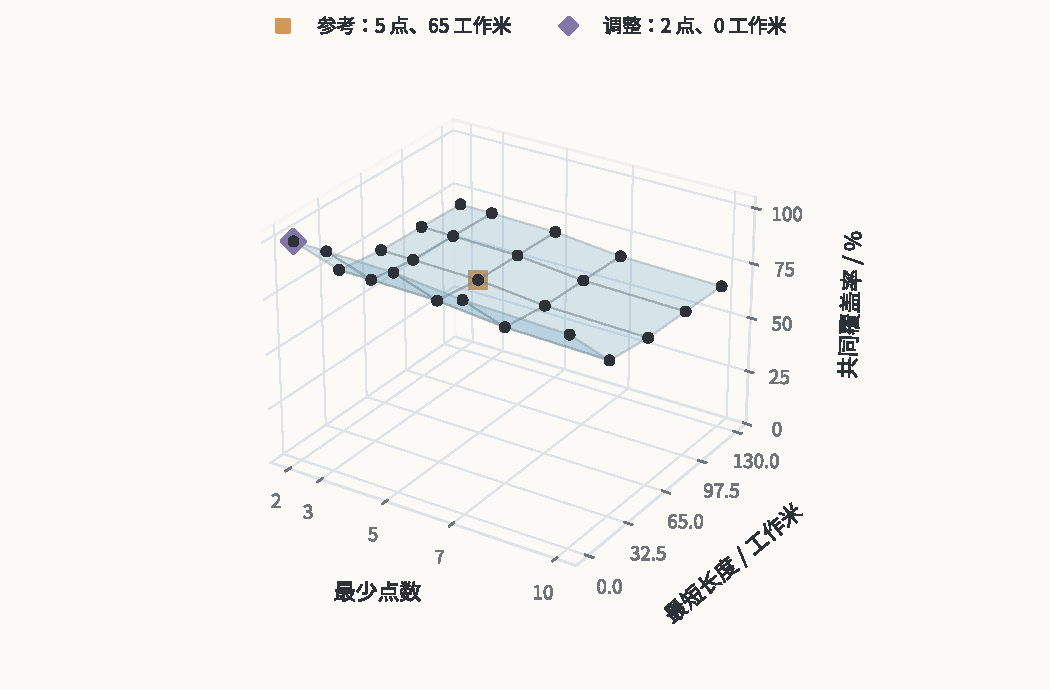
\includegraphics[width=.99\linewidth]{figures/filter_parameter_surface.pdf}
\caption{过滤条件的三维响应网格。分母均为11,777个原始点，黑点为已测试设置；网格面只连接相邻观测，不表示未测位置也有实验结果。杏色方点为参考设置，紫色菱形为后续过滤调整设置。}\label{fig:surface}
\end{figure}

较高的长度门槛会丢弃一批原本包含多个点的片段。取消正长度下限、并将最少点数降到2后，更多原始范围进入后续处理。这里的高度只表示共同覆盖率，不能单凭曲面最高的位置认定真实清洗质量最好；候选还需满足几何、断点和记录保留条件。

在另外120条阶段评估记录中，这一过滤调整全部通过登记保护，53条共同覆盖严格增加。覆盖从8,805增至12,162点，无输出记录从32降到0；显式保留点从2,748增至2,939。新增表达范围远多于新增存储点，说明后续简化仍在发挥作用。

这时仍不能判断两项调整是否都必要，也不知道增加其他规则是否会更好。第\ref{sec:selection}章把点数和长度门槛拆开核验，再检查有依据的组合，而不直接把所有改动叠入最终方案。

\clearpage
\subsection{方向阈值与简化容差的取舍}
放宽方向差阈值，会减少满足双侧删除条件的点。但保留更多点是否改善完整轨迹，还取决于其位置和后续简化，不能由删除数量直接判断。

\begin{figure}[H]\centering
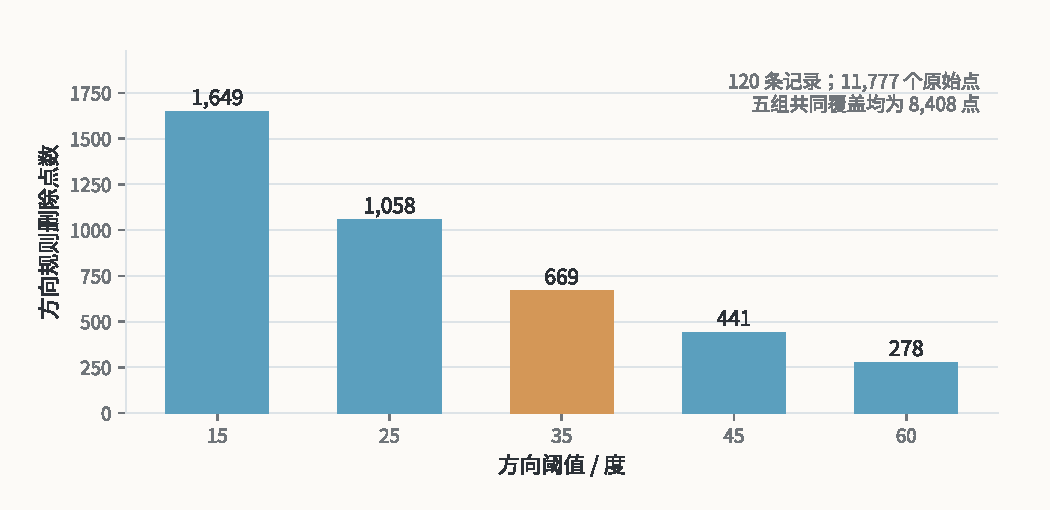
\includegraphics[width=.89\linewidth]{figures/direction_parameter.pdf}
\caption{方向阈值对删除点数的影响。相同开发范围内仅改变方向阈值，参考35度用杏色标出。阈值较宽时删除较少，但五组共同覆盖均为8,408点；这不是噪声准确率曲线。}\label{fig:direction}
\end{figure}

15、35、60度分别删除1,649、669、278点。差异体现了规则的敏感性，但共同覆盖不变，并不意味着几何变化也相同。初轮没有找到能统一替换35度的方向阈值，因而先保留参考，后续只在有明确原始诊断依据时检查条件规则。

DP的取舍更直接：较紧容差通常需要更多保留点，较宽容差可能更精简，但允许更大偏差。图\ref{fig:dp}在同一完整P输入上比较各容差，不将方向删除带来的变化混入压缩收益。

\begin{figure}[H]\centering
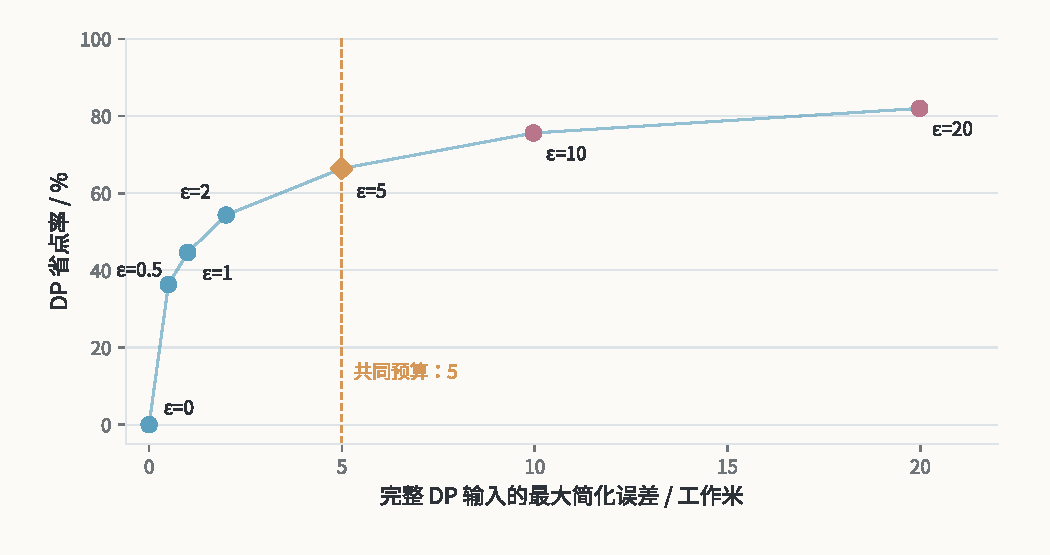
\includegraphics[width=.89\linewidth]{figures/dp_error_saving.pdf}
\caption{相同上游输入上的DP误差与省点率。点旁标记为容差，连线仅连接已测设置。杏色虚线为共同5工作米预算；0是不简化参照，实际超预算的设置用玫瑰色标出。}\label{fig:dp}
\end{figure}

缩小容差带来较低即时误差，却未在共同预算下产生额外省点收益；10、20工作米可展示更宽容差的影响，但实际超出5时不满足最终方案的误差要求。初轮方向与DP单项因此都保留参考设置，而不是为使候选不同而强选新值。

在所测单因素相邻取值之间，也未出现阶段索引、覆盖与各阶段点数全部相同的精确稳定区间。结论仅限这些离散测试，不能由几条相近的平均值推出连续参数范围都稳定。

\subsection{三种操作能否交换顺序}
每一步都改变下一步看到的输入，所以顺序本身也是需要验证的变量。表\ref{tab:orders}比较六种排列。S均包含切分及紧随其后的过滤；D、P在前时没有暗中添加相同的预分段，所有邻接特征在实际变化后重新计算。

\begin{table}[htbp]\centering\small
\caption{六种顺序在120条开发记录上的检查结果}\label{tab:orders}
\begin{tabularx}{\linewidth}{@{}lrrrrY@{}}\toprule
顺序 & 安全失败记录 & 跨断点边 & D跨断点窗口 & P删触发点 & 判断\\\midrule
S-D-P & 0 & 0 & 0 & 0 & 保留参考\\
S-P-D & 0 & 0 & 0 & 0 & 有权衡\\
D-S-P & 46 & 1 & 612 & 1 & 未通过\\
D-P-S & 87 & 1 & 612 & 188 & 未通过\\
P-S-D & 87 & 0 & 0 & 193 & 未通过\\
P-D-S & 87 & 1 & 453 & 193 & 未通过\\\bottomrule
\end{tabularx}
\tabnote{“安全失败”按记录计，后三列按事件计，不能相加。“P删触发点”表示简化删除了原始断点判定所需的观测。表中安全是本实验的共同约束，不是交通安全判断。}
\end{table}

D在S之前时，方向窗口可能跨越本来需要断开的空档。P在S之前时，则可能先移除触发断点的点，令后面的切分看不到原始信息。四种出现实际失败的顺序未继续作为统一改进候选；这类约束拒绝是实验结果，不是需要把方法修到通过的代码错误。

S-P-D在开发及阶段评估中没有出现上述安全失败，但P之后的D会再次改写几何。阶段评估中，S-D-P的共同原始最大偏差约136.118工作米，S-P-D约377.727工作米，而后者P即时误差仍约4.993工作米。局部容差因此不能替代最终几何检查。

这些对照说明三步不能无条件交换，并支持在本次定义、数据与比较规则下保留S-D-P；它们并不意味着所有轨迹任务永远只能使用这一顺序。

\nextchapter\section{LLM辅助处理与建议核验}
\label{sec:llm}

\subsection{一条建议怎样进入实际计算}
参数范围明确后，仍需要判断哪些设置值得尝试。LLM可以根据轨迹诊断提出候选，但建议本身不能说明效果：同样一句“多保留短片段”，可能改善覆盖，也可能保留较大的位置偏差。因此，建议必须转成明确参数，交给同一套工具处理，再用与确定性方案相同的参考检查。

实验使用GPT辅助讨论方法和解释结果，Codex完成实现、运行与资料整理。任务内将规划、执行和核验分成A、B、C三个职责。A依据已有证据提出比较任务；B实际计算与整理；C从原始数据和固定条件核对产物。分段、去噪和DP仍是确定性工具，不各自改名为一个模型。

\begin{figure}[H]\centering
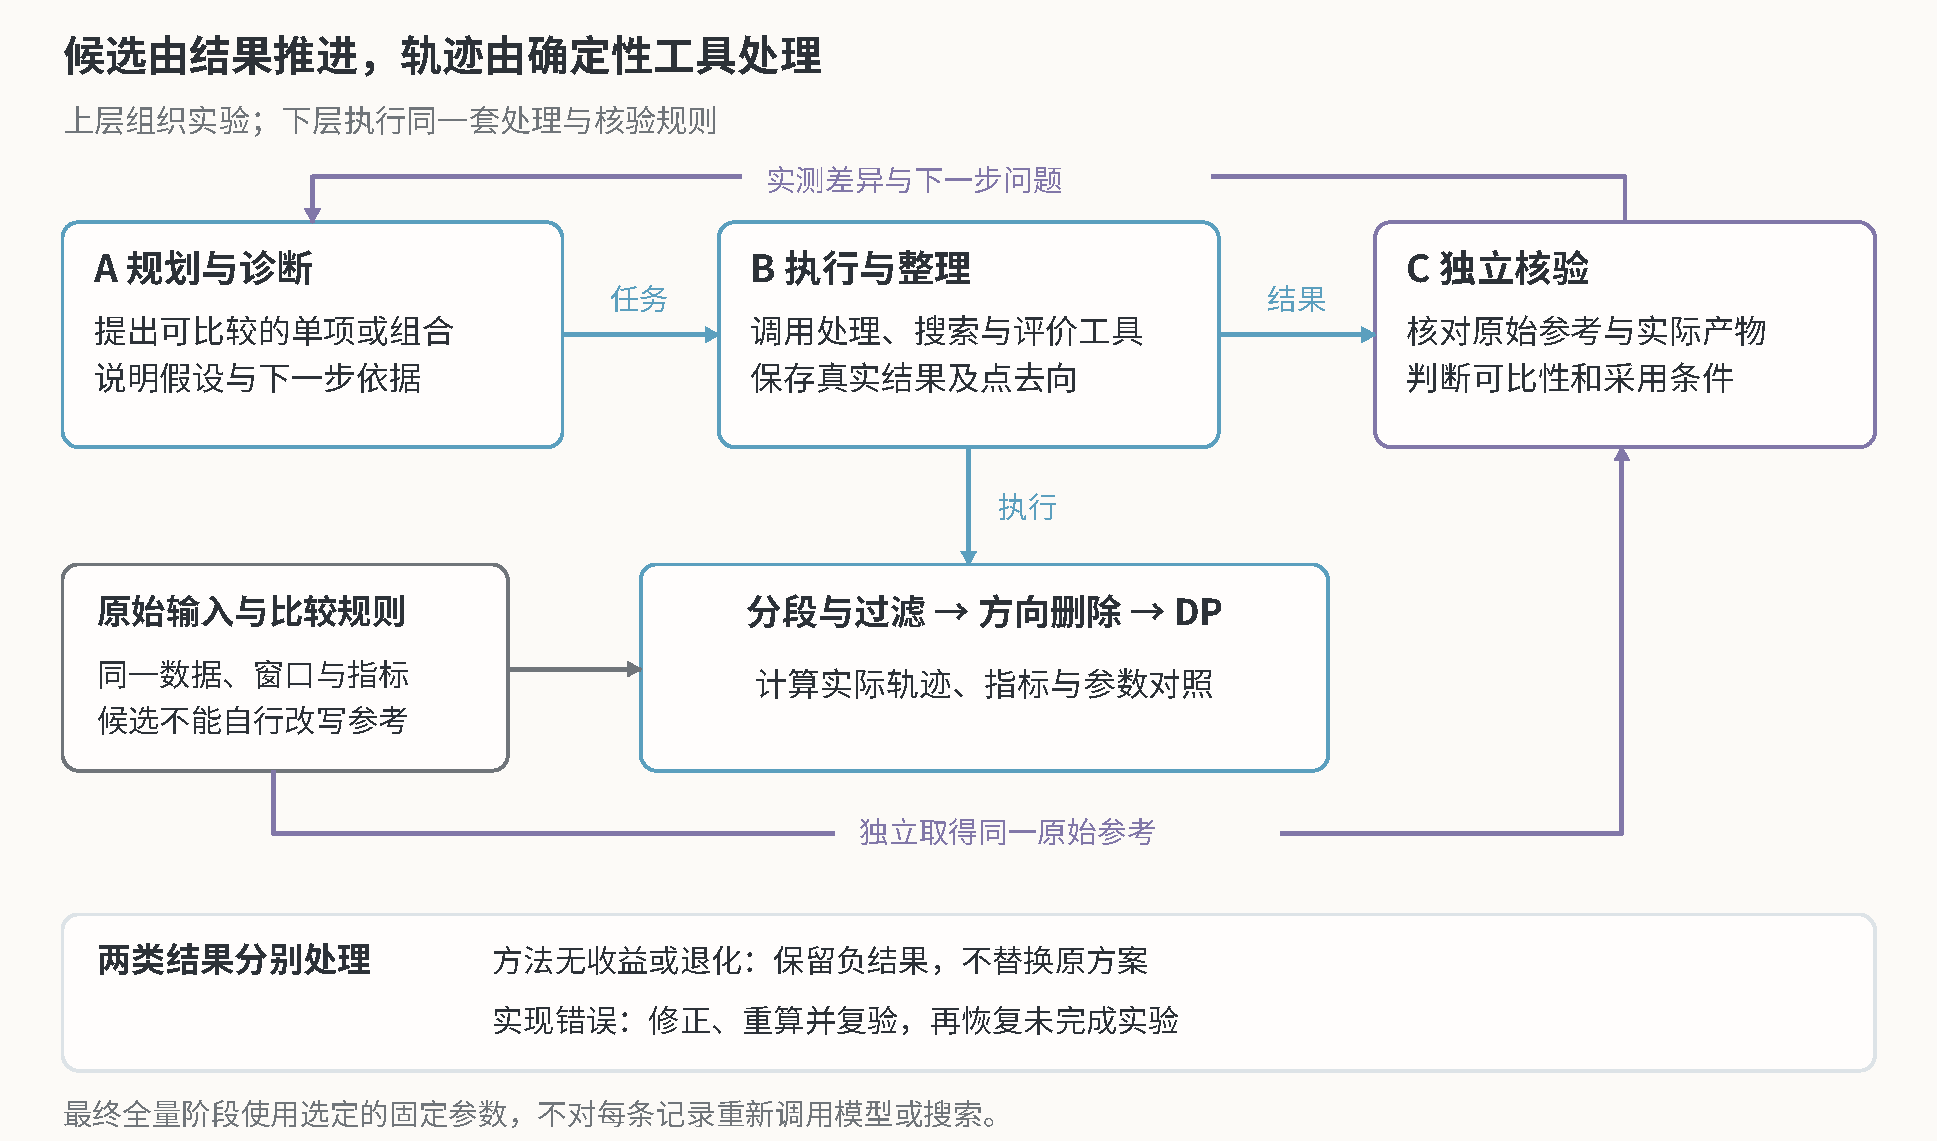
\includegraphics[width=\linewidth]{figures/workflow_structure.pdf}
\caption{实验组织与处理工具的分工。结果核验使用独立取得的原始参考，实测差异返回后续规划。方法无收益与实现错误分别处理；该结构说明实验怎样推进，不表示最终逐记录处理都调用模型。}\label{fig:workflow}
\end{figure}

角色之间传递明确的输入范围、参数、输出和检查结论，而不是只有“帮我优化”的自然语言。执行出错时先修正实现，重新计算受影响结果，再恢复原比较；候选正确执行但无收益时保留负结果，不把它当作必须修到胜出的故障。普通动作在已有范围内完成，改变方法含义或比较目标的问题才需要重新讨论。

这一组织方式服务于整个实验的推进。下面的四模式则比较\textbf{记录级参数决策}怎样使用模型、反馈和记忆，两者不混为一项：治理角色参与代码或报告，不计入“仅确定性搜索”的记录级调用。

\subsection{四种运行方式分别能看到什么}
一次建议是否足够，实测反馈是否有帮助，需要通过不同权限的模式比较。表\ref{tab:mode-definition}列出各模式的差别。它们使用相同数据、基础工具与参数范围，但不强行拥有相同的信息。

\begin{table}[htbp]\centering\small
\caption{四种模式的决策条件}\label{tab:mode-definition}
\begin{tabularx}{\linewidth}{@{}L{32mm}YY@{}}\toprule
模式 & 决策可见信息 & 实际动作\\\midrule
仅LLM建议 & 原始诊断卡、方法和合法参数域 & 一次提议锁定后执行；评分不回传修改该提议\\
仅确定性搜索 & 共同设置及本模式的工具结果 & 按预登记20项配置序列搜索；零记录级模型调用\\
LLM＋搜索 & 原始诊断和自己的实测反馈 & 最多3轮；提出候选、执行、再据结果调整或停止\\
LLM＋记忆＋搜索 & 同上，加冻结示范记忆 & 相同回合与候选上限，额外读取适用经验\\\bottomrule
\end{tabularx}
\end{table}

搜索型模式每条记录最多评价20个候选，反馈轮次的累计上限依次为8、14、20；允许提前停止，所以上限相同不意味着实际计算量相同。仅LLM模式没有搜索机会，不称为等计算量实验。确定性搜索遍历固定序列，LLM可在设定的六参数离散域内提出完整向量；比较的是这些明确策略，而不是完全隔离所有搜索差异后的模型能力。

诊断卡只含必要原始统计，不把完整坐标序列直接塞入模型。每次真实派发最多包含8张卡，分别保存建议与结果。原样建议先接受合法性检查，不先夹到合法范围再统计成功。允许反馈的模式可在剩余预算内修改；仅LLM不能获得隐藏的二次修正。

开发比较采用同一24条记录、各1次独立运行；阶段评估采用另一组共同24条记录、各3次独立运行。表\ref{tab:modes}中的72为$24\times3$次记录观察，不是72条互不相关的轨迹。各次会话与工作记忆重置，模型统一使用\texttt{gpt-6-astra}（medium设置），未固定随机种子。

\begin{table}[htbp]\centering\small
\caption{真实四模式的结果与实际计算量}\label{tab:modes}
\begin{tabular}{@{}llrrrr@{}}\toprule
分区 & 模式 & 改善 / 观察 & 候选评价 & 模型派发 & 批次总时长/秒\\\midrule
开发 & 仅LLM建议 & 8/24 & 36 & 3 & 113.2\\
开发 & 仅确定性搜索 & 9/24 & 480 & 0 & 30.8\\
开发 & LLM＋搜索 & 16/24 & 372 & 9 & 320.8\\
开发 & LLM＋记忆＋搜索 & 17/24 & 330 & 9 & 297.0\\\midrule
阶段评估 & 仅LLM建议 & 15/72 & 109 & 9 & 324.4\\
阶段评估 & 仅确定性搜索 & 27/72 & 1,440 & 0 & 88.6\\
阶段评估 & LLM＋搜索 & 47/72 & 1,080 & 27 & 1,007.0\\
阶段评估 & LLM＋记忆＋搜索 & 47/72 & 954 & 27 & 892.1\\\bottomrule
\end{tabular}
\tabnote{改善指锁定输出通过全部规定保护并有严格改善，不是真实噪声识别成功率。候选评价包含工具参照等实际计量范围；仅LLM的独立参照评价不进入其决策反馈。时间是批次墙钟时间之和，不是每条轨迹的延迟。}
\end{table}

两种允许模型读取反馈的模式，在这组阶段评估中得到较多符合比较条件的输出，但也消耗了更多模型回合。相同记录的重复不是额外独立样本，这些计数不能单独证明任意数据上的总体优势。有效实验共84次可见模型派发；没有用模型调用次数本身作为质量指标。

\subsection{示范记忆是否影响建议与结果}
若经验条目来自待评估记录本身，模型可能只是找回已经知道的答案。因此，情景记忆只用60条独立示范记录建立，并经工具核验后保存。26条在规定比较中获得支持，34条没有新增收益；无收益经验也保留其性质，不改名为成功案例。

检索依据六个原始特征：点数、空间跨度、正时间差中位数的$\log(1+x)$，以及零时间差、重复位置、原始断点比例。尺度只由示范集固定；在相同描述层内取最多3个近邻，排除本记录和已知关联来源。当前运行的短期记录与示范长期记忆分开，评估阶段不写回，也没有另行填入未经来源说明的人类知识条目。

\begin{table}[htbp]\centering\small
\caption{记忆作用的不同观察层次}\label{tab:memory}
\begin{tabularx}{\linewidth}{@{}L{42mm}L{27mm}Y@{}}\toprule
观察对象 & 实际读数 & 能说明什么\\\midrule
带记忆的记录观察收到条目 & 96/96 & 信息实际送入相应上下文\\
决策回合引用有效条目 & 60/241 & 存在可追踪的引用\\
回合满足动作一致判定 & 49/241 & 部分参数与引用内容一致\\\bottomrule
\end{tabularx}
\end{table}

送达、引用和建议变化是不同层次，不能互换分母，也不自动构成质量收益。阶段评估中，带记忆和不带记忆的搜索模式均有47/72个符合条件的输出，但候选和各次运行仍有差异。当前结果既不足以证明记忆的因果质量增益，也不足以证明所有情形等效。最终采用统一参数，不要求在全量处理时逐条重复检索。

\subsection{局部检查合格，为什么仍未采用}
一个具体建议更能说明核验怎样决定取舍。对记录7764，带记忆搜索提出进一步增加空间切分、放宽短段过滤的设置：时间30秒、距离200工作米、最少2点、最短长度0、方向60度、DP容差5工作米。建议同时指出覆盖与保真仍需实测。

参数可以执行，原有122点覆盖也保持不变。但在同一覆盖集合上，最大几何偏差从40.215增至69.145工作米；候选的P即时误差约4.826工作米，仍小于5。它说明\textbf{简化步骤合格，不等于完整处理结果优于参考}，因此该候选没有作为当前采用结果。图\ref{fig:g6}把输入、两条处理路径和不同检查之间的关系展开。

后续使用方向60度、DP容差2的另一提议虽然降低了自身P误差，共同最大偏差仍为42.546工作米，未优于参考。另一个进一步切分的提议丢失了11个原有覆盖点，先违反覆盖条件，此时也不能直接拿不同覆盖集合的最大误差作配对增减。

真实建议并非都无效。记录10232的建议预期方向删除减少，实测由32点降到10点，差值为$-22$，共同最大偏差也降低。预测方向正确、某记录满足比较条件，与跨记录的统一方法成立仍是不同结论。

\FloatBarrier
\begin{landscape}
\thispagestyle{empty}
\noindent{\sffamily\small\color{Muted}智慧城市与位置服务\hfill Experiment Report}\par
\vspace{3mm}
\begin{figure}[H]\centering
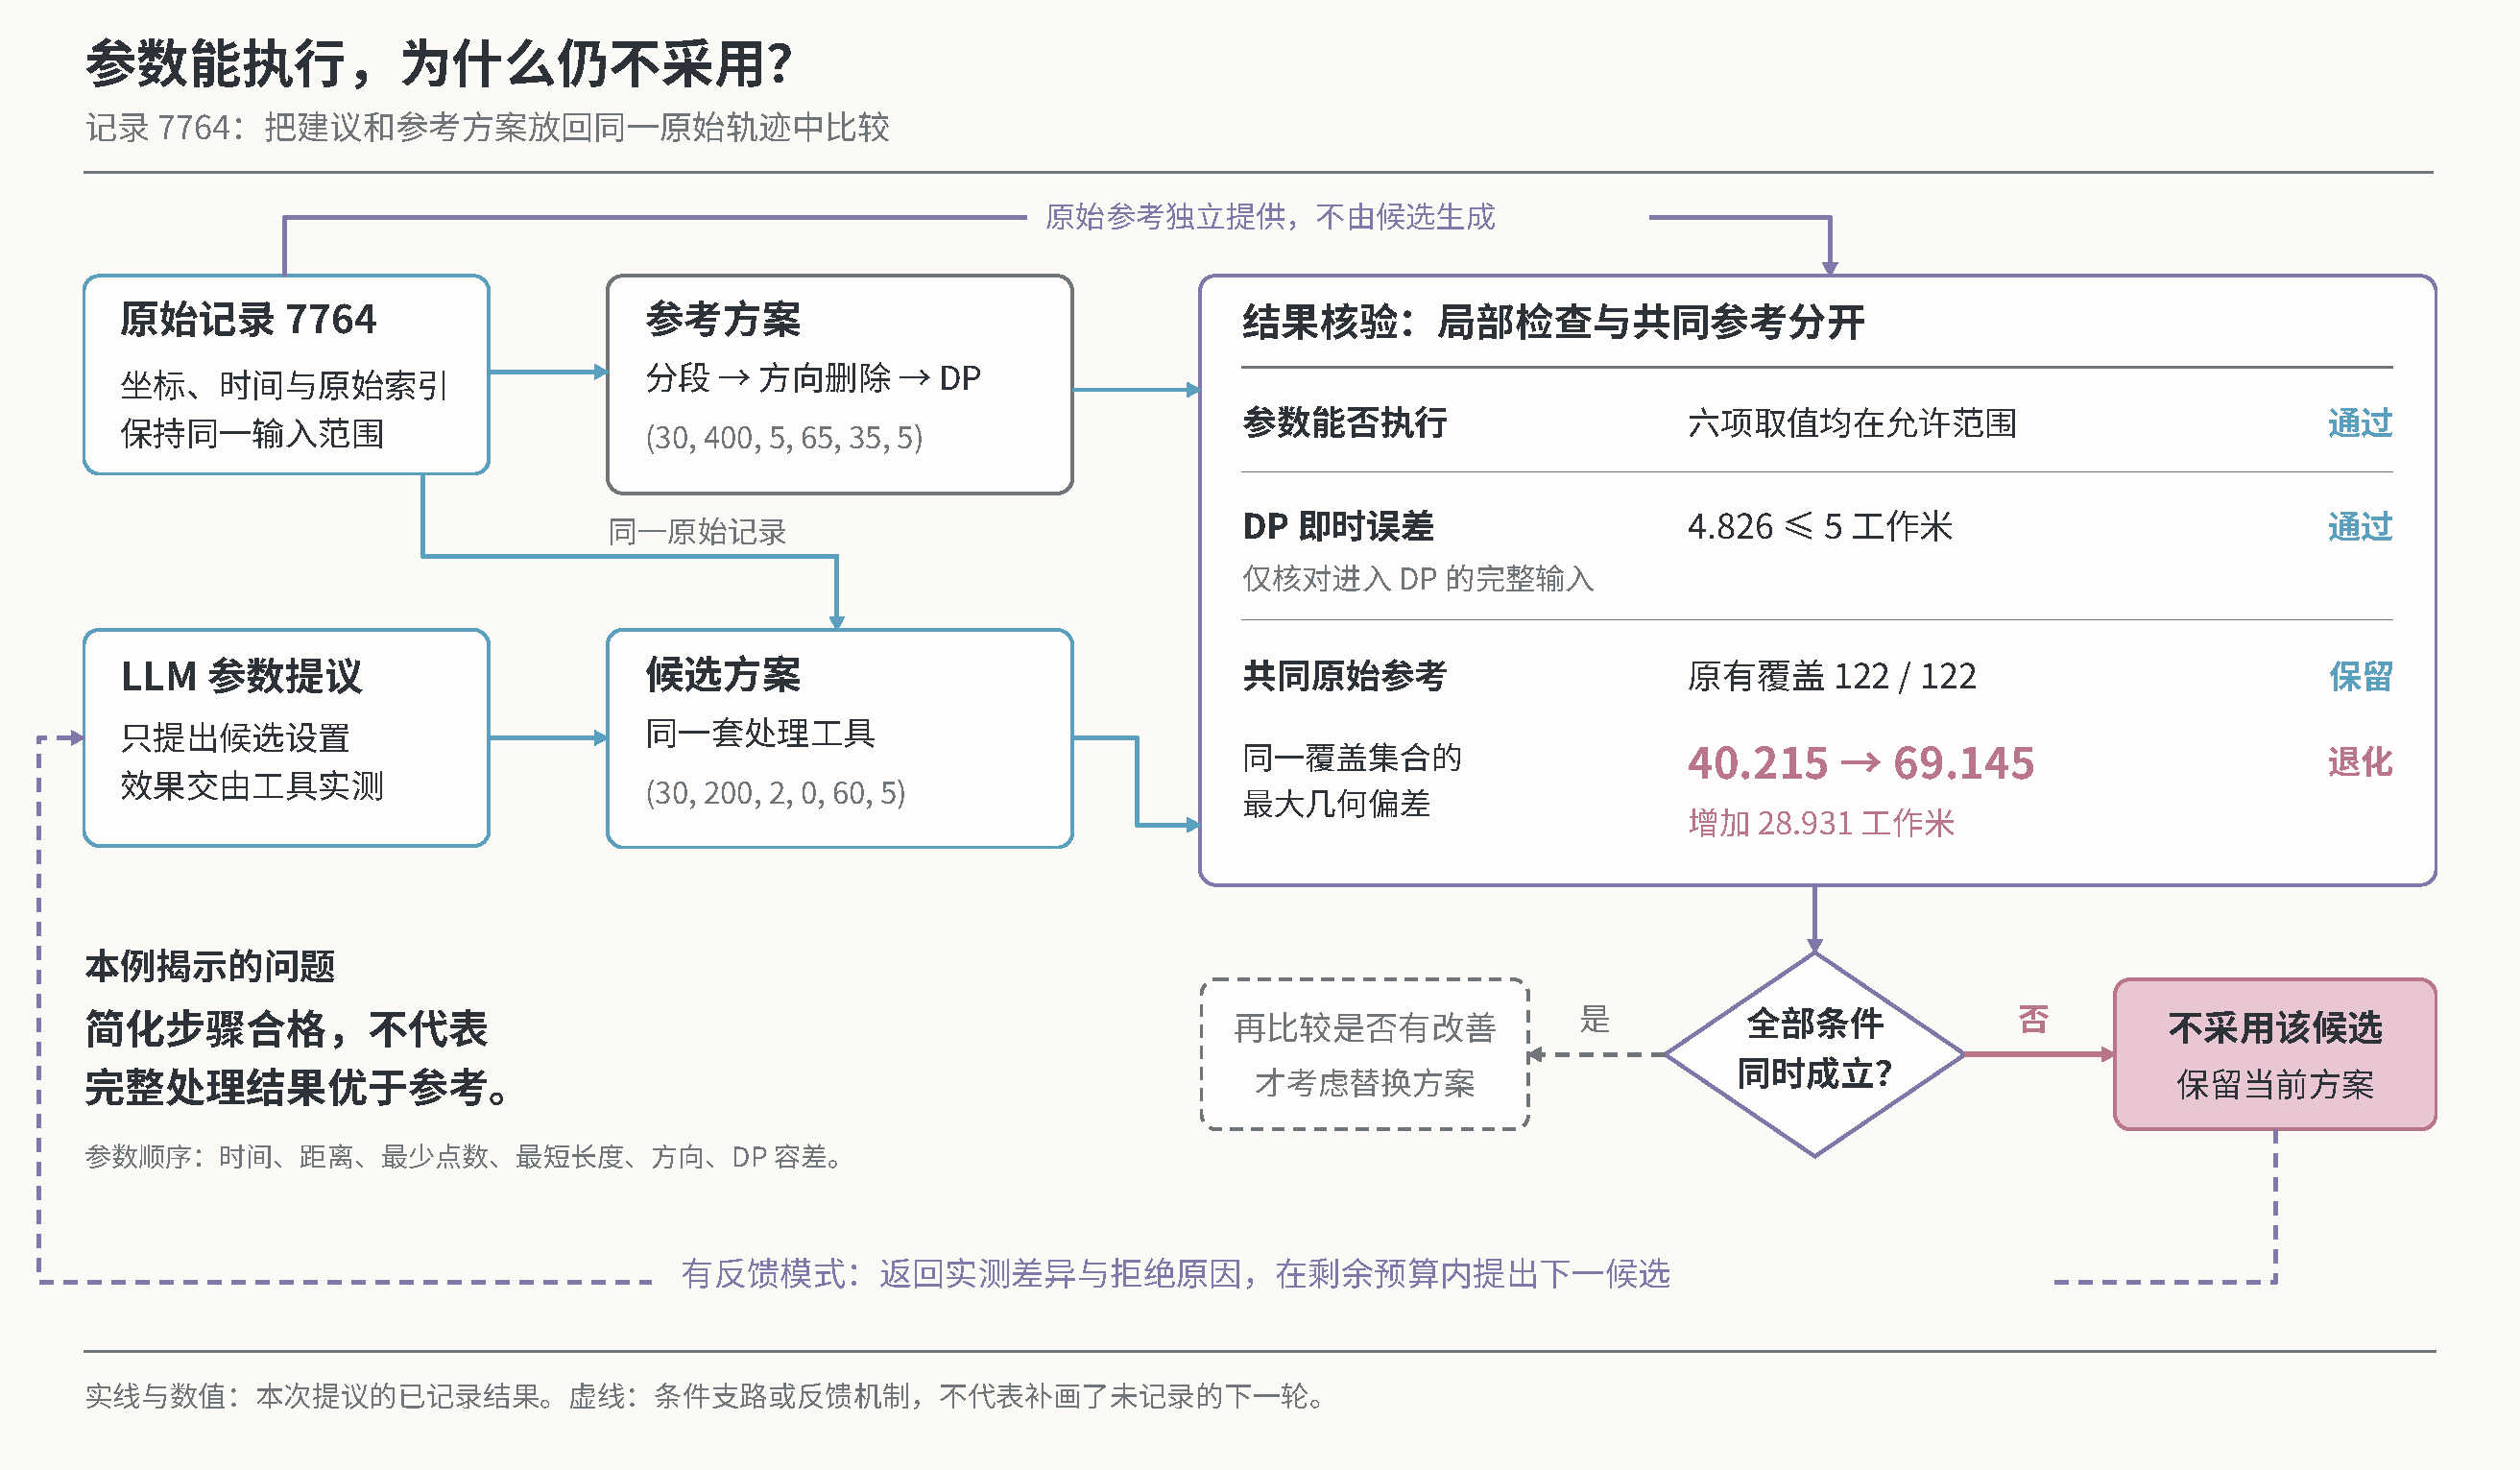
\includegraphics[width=.92\linewidth]{figures/G6A_verification_logic.pdf}
\caption{记录7764的建议核验。原始输入分别供给参考处理、候选处理及独立评价；参数、P即时误差和共同原始几何分开检查。虚线只表示有反馈模式可采用的后续机制，不表示本例发生了图中未列出的新一轮调用。}\label{fig:g6}
\end{figure}
\end{landscape}

\subsection{反例揭示了哪些隐含假设}
真实数据没有噪声真值，不能据删除数量计算误删率。为检查具体数学机制，实验另构造具有已知答案的小型轨迹。表\ref{tab:counterexamples}列出实际运行结果；这些答案仅适用于各自构造，不转移成真实数据标签。

\begin{table}[htbp]\centering\small
\caption{已知答案反例的实测结果与对应认识}\label{tab:counterexamples}
\begin{tabularx}{\linewidth}{@{}L{24mm}Y Y@{}}\toprule
检查问题 & 实际处理结果 & 说明什么\\\midrule
方向与噪声 & 5点正常折返删除2点；5点尖峰删除2点，其中1个预设噪声、1个正常点 & 方向突变不能唯一识别噪声；直角例5点全留也不证明所有转弯安全\\
零值与缺失 & 5点4边中，2条零时间差速度不可用，1条零位移方向不可用 & 不能用速度0、方向0替代不可计算；窗口按定义保留\\
先P后S & 时间间隔例中S-D-P保留4/5点、覆盖100\%；P-S-D无输出 & P即时省点率60\%不能掩盖最终覆盖为0\\
隐藏空间断点 & 两种顺序均留2/3点，P-S-D却有1条跨原始断点边 & 相同点数和覆盖率不足以证明连接关系相同\\
有限线段与等号 & 越界投影距离为$\sqrt2$，正确DP留3点；误差与容差均为1时留2点 & 用有限线段而非延长直线；严格超过才递归\\
全部过滤 & 原始3点仍计入分母，覆盖为0，误差与P省点率不可用 & 无输出不能成为“零误差”的赢家\\
不同clean自证 & 两种方向设置的自身P误差都为0，共同原始最大偏差为0.447214和0 & 各自输入上的低误差不能代替共同参考\\\bottomrule
\end{tabularx}
\end{table}

同理，缺失期间线性插值隐含连续、近似匀速直线运动，但采样空档可能包含停留、转弯或未知路径。实验没有用无依据插值补造轨迹。课程要求的AI批判\cite{teacher}在这里落实为可检查的假设、实际反例与取舍，而不是仅说“不要相信模型”。

基础方法和LLM提议经过相同的处理与评价，保留正例，也保留合法但退化的结果。接下来关注另一个问题：已有单项调整结合后，是否真的带来额外作用。

\nextchapter\section{从单项到组合：改进方案的选择}
\label{sec:selection}

\subsection{分别检查两项过滤调整的作用}
初轮结果支持放宽短段过滤，但最终设置同时改变了点数与长度条件。若不拆开比较，就无法判断收益来自哪一项，也无法确认二者是否都需要保留。因此，在240条已观察记录、23,950个原始点上，分别降低最少点数、取消长度下限，再检查联合调整。

表\ref{tab:development}保留各单项与组合的完整结果。“过滤调整”指最少点数2、最短长度0，其余仍为参考。方向60与DP2、DP10是相应单项，组合只在已有对照上加入指定变化，不同时更换坐标、数据或评价目标。

\begin{table}[htbp]\centering\small
\caption{240条开发记录上的单项与组合。比较参考为相同的原始设置}\label{tab:development}
\begin{tabularx}{\linewidth}{@{}Yrrrrr@{}}\toprule
方案 & 共同覆盖 & 保留点 & D删除 & 保护失败 & 严格改善\\\midrule
参考设置 & 17,213 & 5,349 & 1,427 & 0 & 0\\
仅点数降至2 & 17,379 & 5,479 & 1,427 & 0 & 30\\
仅长度下限为0 & 23,706 & 5,590 & 1,540 & 0 & 77\\
过滤调整 & 23,917 & 5,751 & 1,540 & 0 & 107\\
统一方向60度 & 17,213 & 5,591 & 605 & 3 & 97\\
DP容差2 & 17,213 & 7,295 & 1,427 & 9 & 60\\
DP容差10 & 17,213 & 3,869 & 1,427 & 173 & 0\\
方向条件规则 & 17,213 & 5,434 & 992 & 0 & 41\\
过滤＋方向条件 & 23,917 & 5,836 & 1,058 & 0 & 142\\
过滤＋DP2 & 23,917 & 7,761 & 1,540 & 9 & 149\\
过滤＋DP10 & 23,917 & 4,250 & 1,540 & 178 & 60\\\bottomrule
\end{tabularx}
\tabnote{失败和改善按记录计，均相对参考，二者不是互补计数；有部分改善不意味着全部保护通过。P单项还需在相同输入与共同误差预算下判断压缩收益，不能由本表的改善数直接选出。}
\end{table}

联合过滤调整使共同覆盖增加6,704点，107条记录有严格改善，无输出记录由65降到0。这一收益来自恢复覆盖，而不是在参考已覆盖范围内观察到统一的几何改善。只降低点数，少保留其中6,538个覆盖点；只取消长度下限，少保留211个覆盖点。因此，两项调整均对联合结果有独立作用，但不能把两个单项的改善数直接相加。

这里的较短片段仍可能包含重复位置或位置异常。接受过滤调整表示它减少了按参考条件整段舍弃的信息，后续仍需检查新增范围的偏差；不能将取消长度下限解释为所有短段都已证明有实际出行价值。

\clearpage
\subsection{方向条件规则能否提供额外收益}
统一放宽方向阈值到60度，在开发集上有3条共同几何保护失败，不能直接替换参考。但删除较少的影响可能与采样情况有关，因此进一步测试一个简单规则：若整条记录的原始相邻时间差均可计算，且全部满足$0<\Delta t\leq30$秒，使用60度；其余仍用35度。它只读取原始时间，不按记录编号匹配答案。

开发中满足与不满足该条件的记录各120条。单独使用这一规则，相对参考在41条记录上降低共同最大几何偏差，全部记录通过保护；但它没有恢复过滤调整新增的6,704个覆盖点。两项作用因此具有进一步组合的依据，而非仅因它们都曾出现好结果就直接相加。

“过滤＋方向条件”与参考、两个父方案分别比较。相对过滤调整，覆盖不变，41条几何改善，显式存储增加85点；相对仅方向条件，107条恢复覆盖。相对最初参考共有142条严格改善，是107条覆盖改善与41条几何改善的并集，二者交叠6条。

移去方向规则，失去41条已观察到的几何改善；移去过滤调整，则丢回6,704个覆盖点，使65条重新无输出。这使组合成为开发阶段暂时保留的方案。\textbf{开发中的支持仍需在新的记录上检验，不能直接作为最终采用理由。}

\subsection{DP组合没有因压缩更多而被直接采用}
DP2使即时误差更小，但需要更多输出点；DP10更省点，却可能越过共同预算。为识别P组件自身的作用，每个P变体都与\textbf{完全相同上游、容差为5}的方案比较。

\begin{table}[htbp]\centering\small
\caption{相同P输入上的容差调整：省点收益与误差约束分开判断}\label{tab:p-combination}
\begin{tabularx}{\linewidth}{@{}YrrY@{}}\toprule
比较 & 输出点变化 & 超5预算记录 & 取舍\\\midrule
参考上游：DP2对DP5 & +1,946 & 0 & 未带来压缩收益\\
参考上游：DP10对DP5 & $-1,480$ & 173 & 超出预算\\
过滤调整：DP2对DP5 & +2,010 & 0 & 未带来压缩收益\\
过滤调整：DP10对DP5 & $-1,501$ & 178 & 超出预算\\\bottomrule
\end{tabularx}
\end{table}

过滤与DP2组合虽有覆盖增加，但该增加已由S产生，不能归功于更紧的P容差；它还比相同上游多存2,010点。过滤与DP10则在178条记录上超出预算。两种组合都没有成为更合适的统一方案，较紧容差也不是完整原始几何必然逐点改善的保证。

组合比较增加了一个轻量方向规则及三个组合设置，并完成必要父项和移除检查。另一类删除保护缺少可靠的位移或物理阈值依据，没有为凑齐候选而加入。已有顺序、在线模式也没有新的支持机制，因而不继续无依据扩展。此时保留参考、过滤调整、方向条件及二者组合四个方案，进入独立的选择阶段。

\clearpage
\subsection{组合在新记录上退化之后，怎样取舍}
新选择集含240条记录、24,677点，四个方案在查看结果前已固定。过滤调整在全部记录上保持规定保护，103条共同覆盖严格增加，共增加6,625点。方向条件及其组合虽然仍改善部分记录，却在同三条记录上增大共同最大几何偏差。

\begin{table}[htbp]\centering\small
\caption{四个固定候选在新选择记录上的表现}\label{tab:selection}
\begin{tabularx}{\linewidth}{@{}Yrrrr@{}}\toprule
方案 & 共同覆盖 & 显式保留 & 保护失败 & 严格改善\\\midrule
参考设置 & 18,016 & 5,321 & 0 & 0\\
过滤调整 & 24,641 & 5,784 & 0 & 103\\
方向条件规则 & 18,016 & 5,360 & 3 & 39\\
过滤＋方向条件 & 24,641 & 5,823 & 3 & 138\\\bottomrule
\end{tabularx}
\tabnote{失败和严格改善均相对参考；组合相对过滤调整另有39条几何改善，但其他记录的收益不能抵消三条失败。}
\end{table}

\begin{figure}[H]\centering
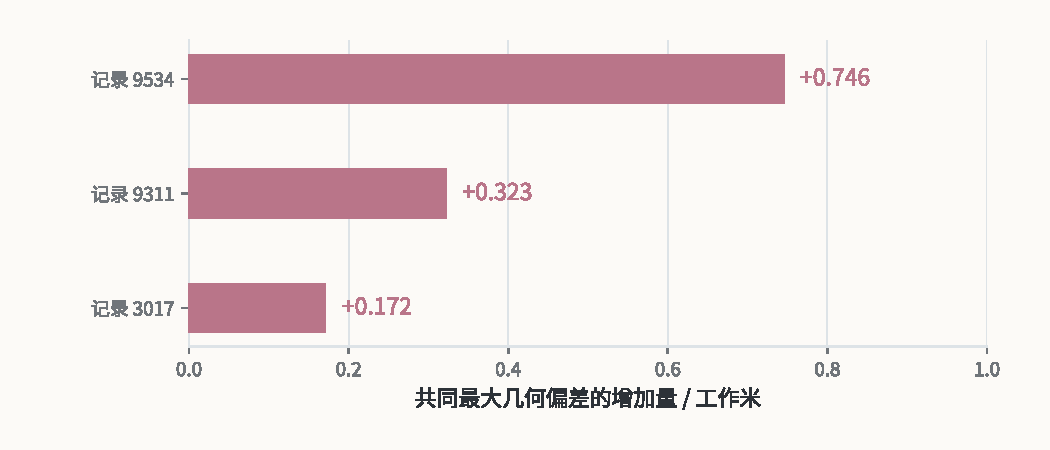
\includegraphics[width=.98\linewidth]{figures/selection_geometry_increase.pdf}
\caption{方向条件加入过滤调整后，三条选择记录的共同最大偏差增加。记录3017、9311、9534的原偏差分别为4.786、3.953、3.718工作米，组合后为4.957、4.276、4.464。图中展示差值，三条均未满足逐记录非退化条件。}\label{fig:selection}
\end{figure}

较宽方向阈值保留了更多点，随后同一个DP5算法在变化后的输入上重新选点。例如记录9311的最终点数仍为10，但原索引27被换为22，共同最大误差由3.953415增至4.276002工作米。两边的P即时误差均不超过5，所以不是DP实现违反定义，而是合法处理后出现真实权衡。

因此，实验没有修改分组条件，也没有从选择集删去这三条记录，而是去掉方向条件，保留较简单的过滤调整。最终仍为S-D-P：时间30秒、距离400工作米、最少2点、最短长度0、方向35度、DP容差5工作米。该决定依据已有比较；下一章再检查其在预留记录上的表现及全量结果。

\nextchapter\section{最终效果与适用边界}
\label{sec:results}

\subsection{选定方案在预留记录上的表现}
选择阶段结束后，最终方案与参考设置一同固定，再处理600条预先保留的记录，共62,284个原始点。它们不用于修改参数、方向条件或记忆。比较仍采用原来的覆盖、共同几何、断点与P预算条件，不因最终结果改变标准。

\begin{table}[htbp]\centering\small
\caption{600条最终确认记录的处理结果}\label{tab:confirm}
\begin{tabularx}{\linewidth}{@{}Yrr@{}}\toprule
读数 & 参考设置 & 最终过滤调整\\\midrule
短段过滤点 & 26,416 & 64\\
方向删除点 & 1,845 & 2,148\\
DP精简点 & 23,032 & 47,958\\
显式保留点 & 10,991 & 12,114\\
共同覆盖点 & 35,868 & 62,220\\
无输出记录 & 255 & 0\\\bottomrule
\end{tabularx}
\end{table}

全部600条通过规定保护，其中349条共同覆盖严格增加、251条覆盖不变。新增覆盖26,352点，显式存储只增加1,123点，表明多数重新进入处理的观测仍由简化后的线段表达。图\ref{fig:confirm-hist}进一步展示增量分布，避免仅用一个总数掩盖记录之间的差异。

\begin{figure}[H]\centering
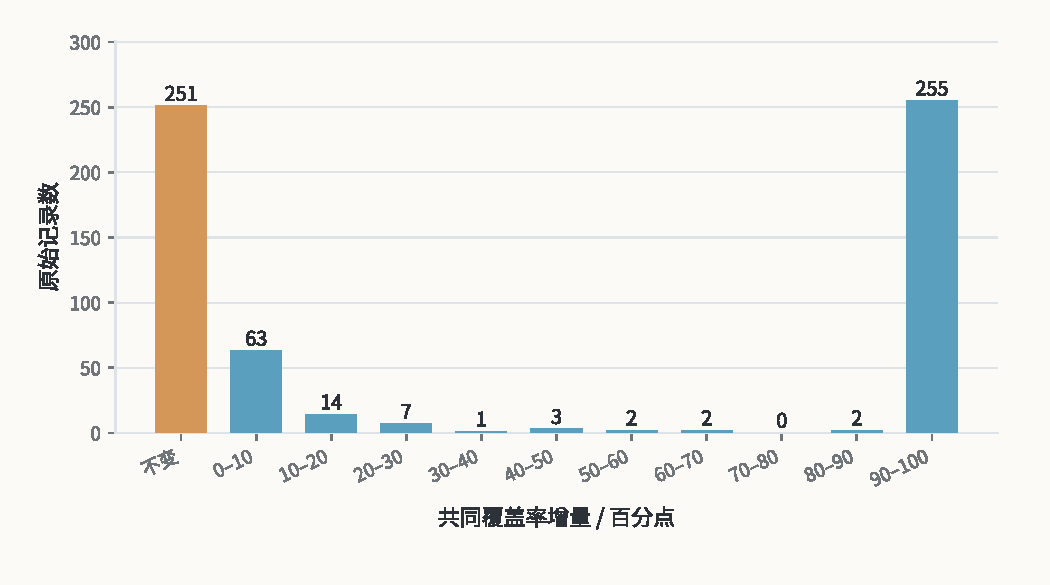
\includegraphics[width=.98\linewidth]{figures/confirmation_gain_histogram.pdf}
\caption{逐记录共同覆盖率的变化。零变化单独列出，其余按10个百分点分箱；统计单位为600条原始记录，100个百分点归入最后一组。覆盖增加不是噪声识别准确率增加。}\label{fig:confirm-hist}
\end{figure}

确认支持所选方案在这批记录和评价条件下采用，预设的参考回退没有触发。这不是再次选取赢家：如果结果不支持改善，就不能继续在同一批确认记录上调整参数。后续全量处理使用已经选定的固定设置，不逐记录调用模型、搜索或记忆。

\subsection{全量处理后，原始点去了哪里}
真实处理全部11,386条记录、1,173,410个点，包括早期开发与各评估分区。全量输出用于描述本数据集的处理结果，不作为另一批未见测试。参考与最终设置均形成25,963个片段，因为时间与距离切分阈值没有改变。

\begin{table}[htbp]\centering\small
\caption{全部轨迹的处理去向与结果}\label{tab:full}
\begin{tabularx}{\linewidth}{@{}Yrr@{}}\toprule
读数 & 参考设置 & 最终过滤调整\\\midrule
S短段过滤点 & 501,511 & 1,199\\
D方向删除点 & 36,056 & 39,732\\
P精简点 & 435,373 & 911,330\\
显式保留点 & 200,470 & 221,149\\\midrule
共同原始覆盖点 & 671,899 & 1,172,211\\
无输出记录 & 4,859 & 0\\
跨原始断点边 & 0 & 0\\\bottomrule
\end{tabularx}
\tabnote{前四项是互斥点去向，每列加总为1,173,410；覆盖与这些去向有重叠，不能再次相加。所有输入点均有终态，无处理失败、未处理记录或实际逐记录回退。}
\end{table}

最终方案相对参考增加500,312个共同覆盖点，只增加20,679个显式保留点。全量逐记录比较中，6,522条有严格改善，其余保持已有保护。图\ref{fig:flow}按同一原始点在两个方案中的状态连线，直接说明新增信息怎样进入后续处理。

\begin{figure}[H]\centering
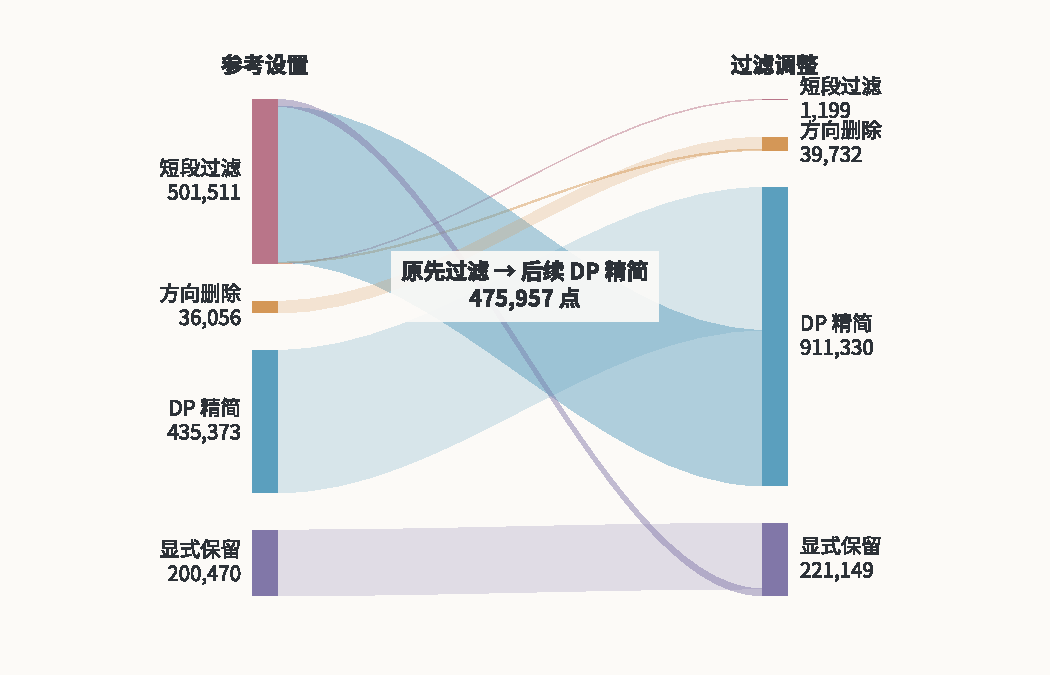
\includegraphics[width=\linewidth]{figures/point_fate_flow.pdf}
\caption{同一批原始点在两个方案中的去向对应。带宽按实际点数绘制；参考过滤掉的点中，475,957点在调整后进入DP精简，而非全部变成存储点。“覆盖”不是互斥终态，故未作为一条额外流加入。}\label{fig:flow}
\end{figure}

每个阶段的索引、坐标和时间均可与原始输入对应，汇总由实际点账本计算。全量的范围、终态和断点条件逐项检查；独立数值核对覆盖随机与边界记录，并保留最大误差案例。评价针对实际输出，而不是只让处理程序再次打印自身声称的统计。

\subsection{覆盖增加与存储量增加为何不同}
DP会用相邻保留点间的线段表示一些没有显式保存的原始点。因此，放宽过滤后，即使大量片段重新进入流程，也不需要原样存储全部点。表\ref{tab:added-cause}进一步将新增覆盖对应回参考过滤的具体原因。

\begin{table}[htbp]\centering\small
\caption{新增500,312个覆盖点原来被过滤的原因}\label{tab:added-cause}
\begin{tabularx}{\linewidth}{@{}Yr@{}}\toprule
参考过滤原因 & 新增覆盖点\\\midrule
仅累计长度不足 & 492,513\\
仅点数不足 & 5,434\\
点数与长度同时不足 & 2,365\\\midrule
合计 & 500,312\\\bottomrule
\end{tabularx}
\end{table}

主要收益来自减少长度下限引起的整段丢失。与此同时，过滤调整后的P输入有1,132,479点，参考只有635,843点，DP省点率分别约80.47\%与68.47\%。这两个百分比使用不同输入，不能写成DP算法提升了约12个百分点。

新的覆盖也不全是有意义的行驶轨迹。近静止观测、短片段乃至位置异常都可能重新被表达。当前结果支持减少参考过滤造成的信息损失；它没有直接评价停留语义、真实路径恢复或噪声识别准确率。

\subsection{较大偏差来自哪一步}
全量P即时最大误差约4.999964工作米，仍在5以内；原始覆盖点到最终折线的最大偏差却约368.707060工作米，两种方案的这一最大值相同。它们使用不同参考集合，因此并不矛盾。

新增覆盖中的最差点是记录352的原始索引105。所在窗口为104--107，共4点，累计长度约809.444工作米。参考因点数少于5过滤它，并非长度太短。过滤调整保留该段后，D删除105；P的输入与输出均为104、106、107，局部没有再删点。

\begin{figure}[H]\centering
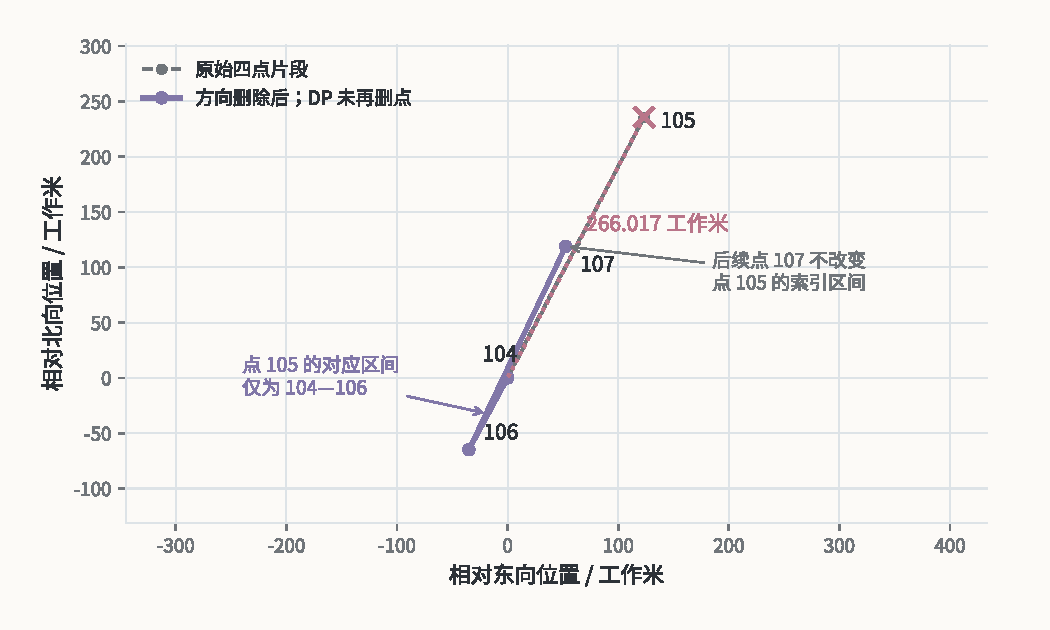
\includegraphics[width=.95\linewidth]{figures/boundary_record352.pdf}
\caption{记录352的局部边界案例。灰色虚线为原始四点片段，紫线为最终输出，玫瑰色虚线表示原始点105到对应最终线段的偏差。坐标只平移到104点，保持等比例；D删除的点不属于P即时输入。}\label{fig:boundary}
\end{figure}

点105按原始索引由104与106夹住，因此只在这条线段上计算偏差，不改取后续的106—107段。其距离为266.016754工作米。这个例子没有违反DP的输入误差定义，却说明覆盖恢复与原始形状完整保留仍然不同。现有资料也不能断言105是真实噪声或真实折返。保留这一案例，比只展示平滑后的成功轨迹更能限定最终结论。

全量坐标核对延续同一数学模型，没有把7条早期试运行的结果直接当成全域数值保证。独立转换核对用于检查实现，实际阈值敏感性另行检查；二者都不能反推源坐标基准。上述几何读数应当继续按工作米理解。

\nextchapter\section{讨论与总结}

\subsection{哪些改进得到本次结果支持}
这次实验并未得到一条“步骤更多就更好”的路线。单项比较表明，参考短段过滤丢失了较多仍可表达的原始范围；将点数与长度门槛分别检查后，两项调整都有作用。方向条件与过滤的组合曾在开发数据上取得额外收益，但新选择数据的三条几何退化使它退出，最终采用了更简单的S-D-P设置。

冻结后的600条记录支持这一选择，全量结果也显示覆盖增加明显大于存储量增加。主要贡献是降低参考过滤带来的信息损失，而不是发明新的DP算法。时间30秒、距离400工作米、最少2点、最短长度0、方向35度和DP5工作米，是在这次离散候选、数据与比较条件下选出的设置，不是对所有轨迹的最优参数承诺。

对LLM的使用也遵循同样的结果标准。建议会转成真实计算，合法性、局部误差和完整几何分开检查；允许反馈的模式据实测继续，而不是由模型自行宣布有效。记忆虽有实际送达与引用，现有比较未证明其因果质量收益。最后保留固定处理策略，并不否定工作流在组织实验、核验和修复中的作用，但不能据此宣称所有Agent组件都带来了可分离的效果提升。

\subsection{哪些问题尚不能由现有数据回答}
最大的限制是没有真实道路、运动类型和位置误差标签。共同原始参考能够帮助发现处理过程的信息损失，却不能区分所有噪声与真实运动；新增覆盖也可能包含较大偏差。方向反例和记录352的局部现象说明，单个算法的保证不能替代整条链的质量判断。

坐标基准及采样来源说明不完整，记录之间的真实个体独立性也不能确认。因此，本文结论限定于固定数学工作平面与所处理数据；分层样本结果、重复模型运行和全量生产分别解释，不相互替代。

实验采用有限参数域和少量有依据的结构调整，并未穷尽所有策略。它形成的主要认识是：\textbf{先让每项操作与评价可核对，再用共同条件下的实际结果决定取舍。}复杂候选可以被否定，原有设置也可以被调整；真正需要保留的是能够被数据支持的部分，而不是预先设想的方案形态。

\FloatBarrier
\vspace{6mm}
\begingroup\small
\begin{thebibliography}{9}
\addcontentsline{toc}{section}{参考文献}
\bibitem{teacher} 董宜滔. 实验课安排和考核方式：轨迹数据质量提升[课程课件]. 华东师范大学，2026.
\bibitem{proj-cart} PROJ contributors. Geodetic to cartesian conversion[技术文档]. \url{https://proj.org/en/stable/operations/conversions/cart.html}.
\bibitem{proj-topo} PROJ contributors. Geocentric to topocentric conversion[技术文档]. \url{https://proj.org/en/stable/operations/conversions/topocentric.html}.
\bibitem{cawley} Cawley G C, Talbot N L C. On over-fitting in model selection and subsequent selection bias in performance evaluation[J]. Journal of Machine Learning Research, 2010, 11: 2079--2107.
\end{thebibliography}\endgroup
\nextchapter\appendix\section{计算与复现补充}
\label{sec:appendix}

\subsection{局部工作坐标的计算}
为使距离计算统一，实验固定椭球半长轴$a=6\,378\,137$米、反扁率$1/f=298.257223563$，令高度$h=0$。固定局部原点为$(\lambda_0,\phi_0)=(121.343555^\circ,31.3561015^\circ)$，没有根据候选得分移动原点。

将经纬度转成弧度，设$e^2=f(2-f)$、$N_\phi=a/\sqrt{1-e^2\sin^2\phi}$，先计算地心直角坐标：
\begin{align*}
X&=(N_\phi+h)\cos\phi\cos\lambda,\\
Y&=(N_\phi+h)\cos\phi\sin\lambda,\\
Z&=[N_\phi(1-e^2)+h]\sin\phi.
\end{align*}
减去原点的地心坐标后，取局部东、北方向：
\begin{align*}
E&=-\sin\lambda_0\Delta X+\cos\lambda_0\Delta Y,\\
N&=-\sin\phi_0\cos\lambda_0\Delta X-\sin\phi_0\sin\lambda_0\Delta Y+\cos\phi_0\Delta Z.
\end{align*}
该数学转换与PROJ文档中的地理坐标到地心坐标、固定原点地心到局部坐标的定义对应\cite{proj-cart,proj-topo}。原始坐标保持不变，图中的“相对位置”仅作平移。时空图第三轴为相对时间，不是高度，也不加入二维距离或DP误差计算。

初轮307条、30,992点的独立PROJ路径核对，最大坐标差约$4.82\times10^{-10}$工作米。该范围内1,594,527个记录内点对的ENU距离与相应椭球测地距离最大绝对差约3.503584米、最大相对差约0.015054\%。前者检查计算实现，后者描述模型近似，两者都不是仪器测量误差。实际处理阶段的敏感性检查在已检验范围内未发现登记动作变化，不能据此推广为源坐标精度已知。

\subsection{读数与实验的复算入口}
作业提供两份完成版Notebook：基础本对应轨迹预处理、参数和顺序实验，系统本对应LLM辅助与评价。两者调用共同的处理与指标实现，使用项目相对路径。默认完整复算从原始输入和固定设置重建轨迹、读数与图表，不新增模型调用；涉及模型建议时读取当时保存的真实响应，再运行确定性工具。

重新发起模型实验使用单独的显式入口，产生新的响应和结果，不能要求随机模型逐字复现旧回答。原始数据、各阶段点索引、参数表、真实建议和复现说明随工程保留；本报告用表图解释主要发现，不将文件校验和运行日志重复列入正文。

\end{document}
